% \begin{app}[Vectoriële kinematica]{Vectoriële kinematica}

% % \begin{itemize}
% %     \item $ \Vec{r} = r\Vec{u} $
% %     \item $ \Vec{v} = \dfrac{d\Vec{r}}{dt} $
% %     \item $ \Vec{a} = \dfrac{d\Vec{v}}{dt} = \dfrac{d^2\Vec{r}}{dt^2}$
% % \end{itemize}

% % % \vspace{0.5cm}

% % % \noindent Hieruit volgt dan logischerwijs ook: 

% % % \vspace{0.5cm}

% \centering
% \def\arraystretch{2.5}
% \begin{tabular}{c|c|c}
%      & $ \Vec{v} $ & $ \Vec{a} $ \\ \hline 
%      gem &  $ \Vec{v}_{gem} = \dfrac{\Delta \Vec{r}}{\Delta t} $ & $ \Vec{a}_{gem} = \dfrac{\Delta \Vec{v}}{\Delta t} $ \\ \hline
%      ogb & $ \Vec{v}  
%      % \lim_{\Delta t \to 0} \dfrac{\Delta \Vec{r}}{\Delta t}  
%      = \dfrac{d\Vec{r}}{dt}$ & $ \Vec{a} = 
%      % \lim_{\Delta t \to 0}\dfrac{\Delta \Vec{v}}{\Delta t} = 
%      \dfrac{d\Vec{v}}{dt} $ 
% \end{tabular}

% \end{app}

\begin{pro}[Nuttige vergelijkingen bij constante versnelling]{Nuttige vergelijkingen bij constante versnelling}
    \vspace{-0.3cm}
    De volgende vergelijkingen kunnen gebruikt worden wanneer de versnelling constant is: $a = \dfrac{dv}{dt} = \text{cst}$:
    \begin{enumerate}
        \item $ r = r_{0} + v_{0}t + \tfrac{a}{2}t^2 = r_{0} + \overline{v}t$
        \item $ v = v_0 + at $ 
        \item $ \overline{v} = \dfrac{v + v_0}{2}$
        \item $ v^2 = v_0^2 + 2a(r-r_0) $
        % \begin{itemize}
        %     \item Dit kan je verkrijgen door (2) en (3) te substitueren in (1).
        % \end{itemize}
    \end{enumerate}
    \vspace{-0.3cm}
\end{pro}

\begin{app}[Projectielbeweging]{Projectielbeweging}
    Bij een projectielbeweging heeft het systeem horizontaal een constante snelheid (eenparige beweging) en verticaal een constante versnelling (eenparig versnelde beweging). In de volgende tabel zijn de formules samengevat: 

    \vspace{0.3cm}

    \begin{minipage}{.66\textwidth}
        \begin{center}
            \def\arraystretch{2}
            \begin{tabular}{c|c|c}
                & $x$ & $y$ \\ \hline
                $ r $ & $ x_0 + v_{x,0}t $ & $ y_0 + v_{y,0}t - \frac{gt^2}{2} $ \\ \hline
                $ v $ & $ v_{x,0} $ & $ v_{y,0} - gt $  \\ \hline
                $ a $ & $ 0 $ & $ -g $ 
            \end{tabular}
        \end{center}

        \vspace{0.3cm}
        % Ik ben ook niet trots op deze code, maar het werkt
        \hspace{-0.5cm}\noindent Hieruit kunnen we volgende formules halen: 

        \hspace{-0.5cm}\begin{minipage}{.43\textwidth}
            \begin{align*}
                x(t) &= v_{x,0}t \\
                y(t) &= v_{y,0}t - \frac{gt^2}{2}
            \end{align*}
        \end{minipage} \hspace{-0.5cm}$\longrightarrow$
        \begin{minipage}{.43\textwidth}
            \vspace{-0.2cm}
            \begin{equation*}
                y(x) = \frac{v_{y,0}}{v_{x,0}}x - \frac{g}{2v_{x,0}^2}x^2
            \end{equation*}
        \end{minipage}
        % \vspace{0.3cm}
    \end{minipage}
    \hspace{-1cm}\begin{minipage}{.4\textwidth}
        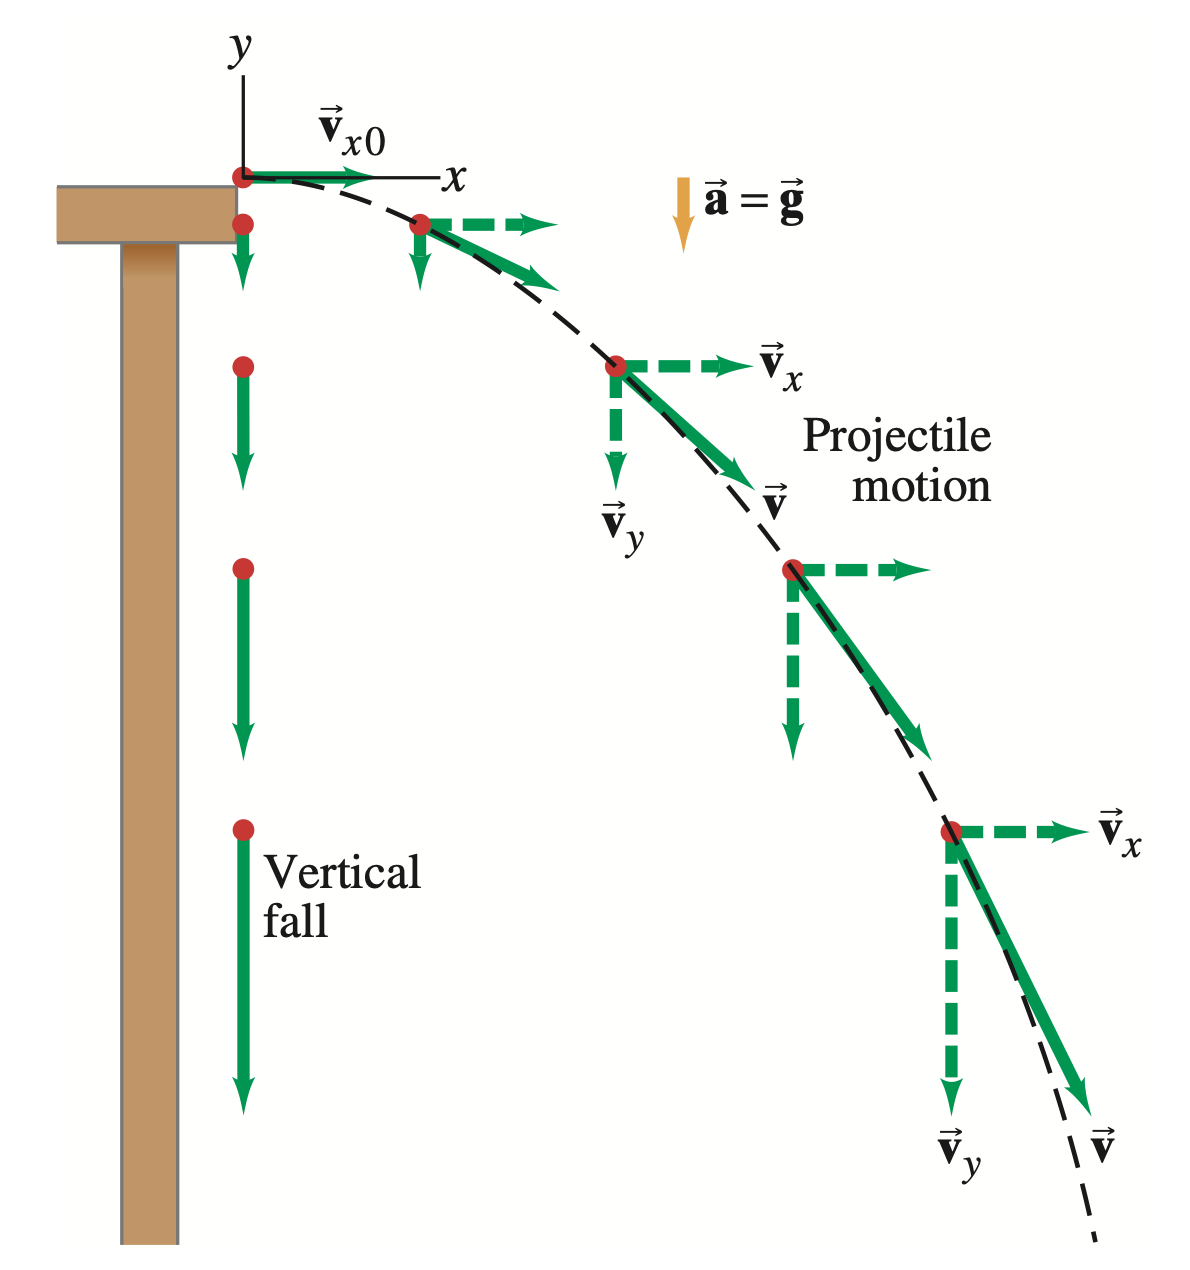
\includegraphics[scale = 0.255]{Images/Kinematica/Projectielbeweging.png}
    \end{minipage}

    \vspace{0.3cm}

    \noindent Deze formule bepaald de volgende parabole projectielbaan:
    \begin{center}
        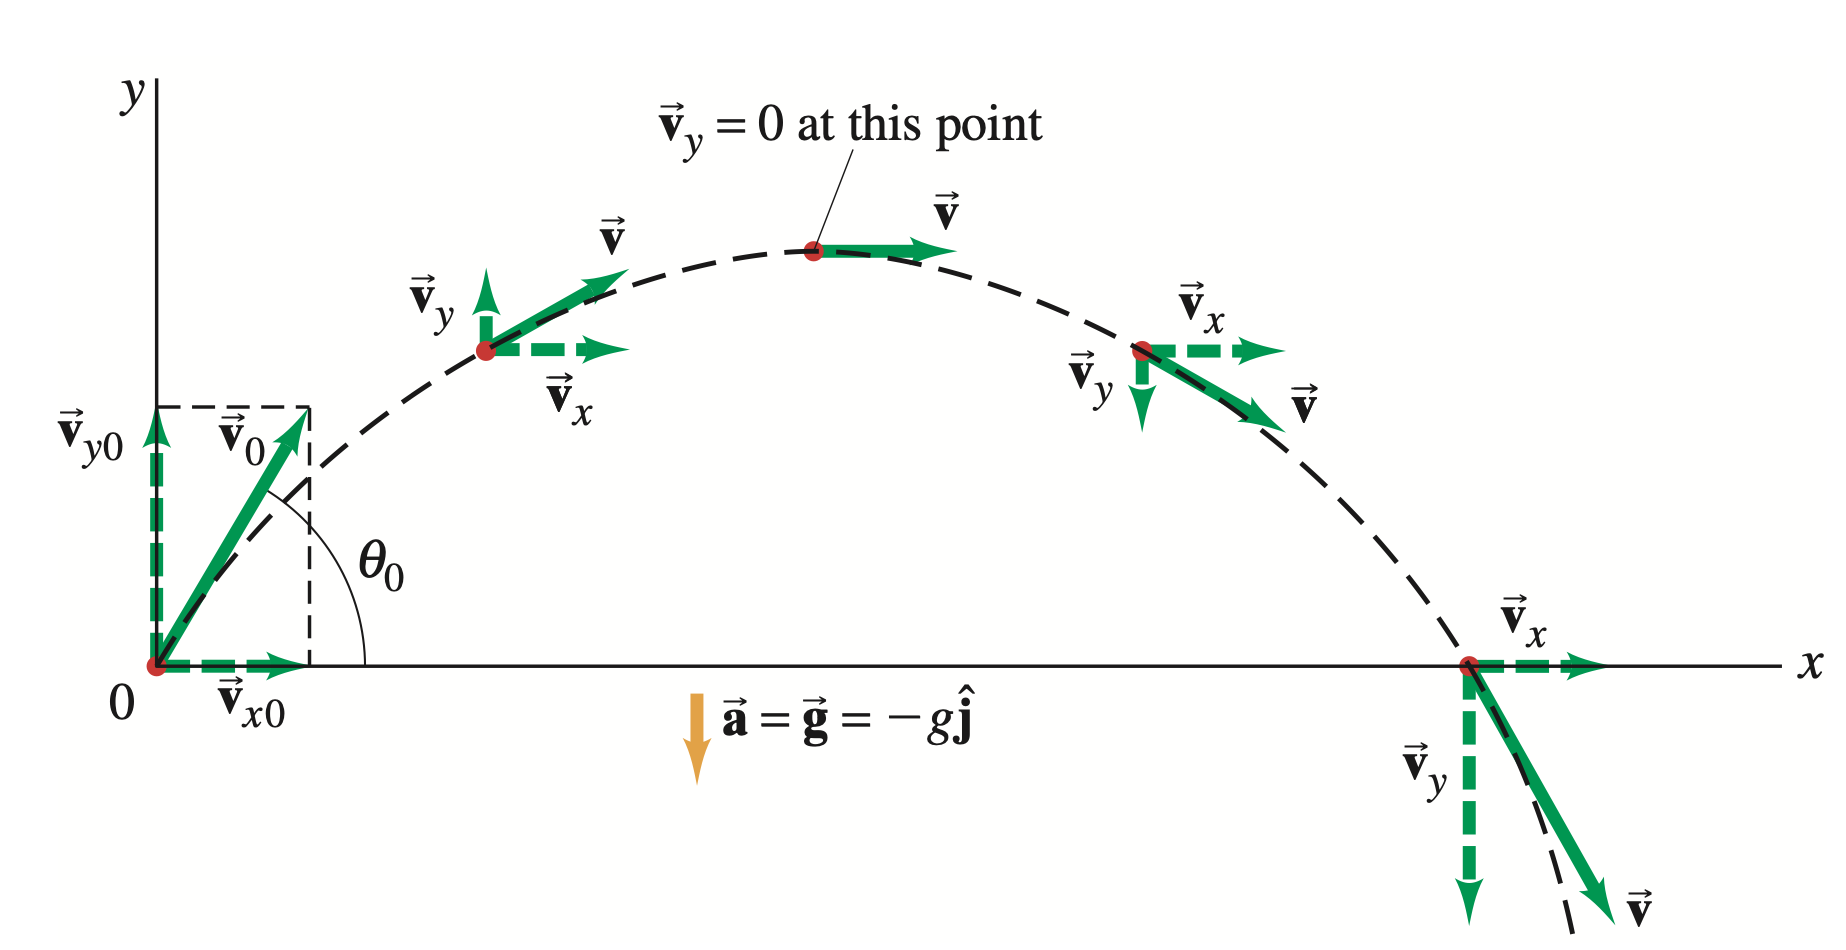
\includegraphics[scale = 0.28]{Images/Kinematica/Projectielbaan.png}
    \end{center}
\end{app}
